\documentclass[11pt]{article}
\usepackage[a4paper,margin=0.90in]{geometry}
\usepackage{amsmath,amssymb,amsthm,mathtools}
\usepackage{booktabs,array}
\usepackage{graphicx}
\usepackage{xcolor}
\usepackage[hidelinks]{hyperref}
\hypersetup{
  pdftitle={Every Spectral Switch Costs Memory},
  pdfauthor={Lluis Eriksson},
  pdfsubject={Sharp robust Wigner--Smith speed limits for passive quantum networks}
}
\usepackage[nameinlink,capitalise]{cleveref}
\usepackage{microtype}

\newtheorem{theorem}{Theorem}[section]
\newtheorem{proposition}[theorem]{Proposition}
\newtheorem{lemma}[theorem]{Lemma}
\newtheorem{corollary}[theorem]{Corollary}
\theoremstyle{definition}
\newtheorem{definition}[theorem]{Definition}
\newtheorem{example}[theorem]{Example}
\theoremstyle{remark}
\newtheorem{remark}[theorem]{Remark}
\newtheorem{limitation}[theorem]{Limitation}

\newcommand{\C}{\mathbb{C}}
\newcommand{\T}{\mathbb{T}}
\newcommand{\D}{\mathbb{D}}
\newcommand{\diag}{\operatorname{diag}}
\newcommand{\rank}{\operatorname{rank}}
\newcommand{\tr}{\operatorname{tr}}
\newcommand{\ran}{\operatorname{ran}}
\newcommand{\dd}{\mathrm{d}}
\newcommand{\e}{\mathrm{e}}
\newcommand{\mcdeg}{\deg_{\mathrm{McM}}}
\newcommand{\snorm}[1]{\left\lVert#1\right\rVert_1}
\newcommand{\onorm}[1]{\left\lVert#1\right\rVert_{\mathrm{op}}}

\title{Every Spectral Switch Costs Memory:\\
Sharp Robust Wigner--Smith Speed Limits\\
for Passive Quantum Networks}
\author{Lluis Eriksson}
\date{10 August 2026}

\begin{document}
\maketitle

\begin{abstract}
Exact interpolation can force the internal degree of a passive network, but
laboratory calibrations are approximate.  We prove a sharp frequency-domain
speed limit that needs neither exact zeros nor analytic continuation away
from the measured frequency axis.  Let $S(\e^{\mathrm{i}\theta})$ be an
absolutely continuous unitary scattering path with positive Wigner--Smith
generator
\[
 Q(\theta)=-\mathrm{i}S(\e^{\mathrm{i}\theta})^*
 \partial_\theta S(\e^{\mathrm{i}\theta})\succeq0.
\]
A fixed $k$-dimensional input subspace is routed approximately into one
output sector at one end of a frequency arc and into its orthogonal
complement at the other.  If the two amplitude leakages are
$\varepsilon_p,\varepsilon_s$ and
\[
 \alpha=\left[\frac{\pi}{2}-\arcsin\varepsilon_p
                      -\arcsin\varepsilon_s\right]_+,
\]
then every such transition obeys
\[
 \int_I\tr Q\,\dd\theta\geq2k\alpha,
 \qquad
 \int_I\lambda_{\max}(Q)\,\dd\theta\geq2\alpha.
\]
Consequently a transition across width $\Delta$ forces peak trace delay at
least $2k\alpha/\Delta$ and peak proper delay at least
$2\alpha/\Delta$.  For disjoint arcs the costs add.  If $S$ is rational
inner of McMillan degree $n$, $\int_\T\tr Q=2\pi n$; hence $M$
alternating pass/stop pairs imply
\[
 \boxed{\displaystyle
 n\geq \frac{2Mk}{\pi}
 \left[\frac{\pi}{2}-\arcsin\varepsilon_p
                      -\arcsin\varepsilon_s\right]_+.}
\]
At zero error this is $n\geq Mk$.  A $2k$-port interferometric family of
degree $Mk$ saturates the global law exactly and saturates both local laws
for every admissible error pair, proving all constants optimal.  The proof
combines canonical-angle geometry on the Grassmannian with two sharp
off-diagonal inequalities for positive Wigner--Smith matrices.  A
measurement-error corollary converts finite scattering tomography directly
into certified degree and delay lower bounds.  Reproducible audits include
2,048 random positive matrices and 512 random Blaschke--Potapov products.
\end{abstract}

\noindent\textbf{Keywords:} Wigner--Smith time delay; McMillan degree;
passive quantum networks; approximate spectral routing; Grassmannian;
rational inner functions; robust interpolation.

\section{The result in one picture}

A passive network may direct the same input channel toward different output
sectors at different frequencies.  This behavior underlies multiplexing,
reservoir selection and frequency-dependent placement of an operational
system--environment boundary.  The ideal specification is binary:
\[
 \text{pass: input subspace lies in sector }A,
 \qquad
 \text{stop: it lies in sector }B=A^\perp.
\]
Real data only certify small leakage.  The question is therefore not how
many exact transmission zeros a transfer function has, but how far its
\emph{output subspace must travel} as frequency changes.

The answer is a geometric action law.  Write $\mathcal X(\theta)$ for the
rank-$k$ output subspace generated by the chosen inputs.  A pass-to-stop
transition separates the endpoint subspaces by at least $k\alpha$ in the
trace-angular Grassmann metric.  The positive Wigner--Smith matrix supplies
the velocity, but positivity makes motion expensive: at most one half of
$\tr Q$ can appear in the off-diagonal block that moves $\mathcal X$.
Thus
\begin{equation}\label{eq:headline}
 \underbrace{2k\alpha}_{\text{required routing motion}}
 \ \leq
 \underbrace{\int_I\tr Q}_{\text{Wigner--Smith memory on the arc}}.
\end{equation}
The largest eigenvalue of $Q$ controls the same transition without the
factor $k$.  Narrow transitions consequently require large proper delays.

The distinction from the exact calibration law in
\cite{ErikssonMemory2026} is fundamental.  That law counts zeros and gives
one unit of degree per exactly lossless direction, even when the calibrated
frequencies cluster.  Approximate samples alone cannot support such a count.
The present result replaces exactness by an ordered routing pattern:
approximately pass and approximately stop must alternate.  It then recovers
the exact coefficient at zero error and remains quantitative at finite
error, using only boundary data.

Our contributions are:
\begin{enumerate}
 \item a nonrational action theorem for every absolutely continuous unitary
 path with $Q\succeq0$;
 \item additive bounds over arbitrary disjoint frequency arcs;
 \item a robust McMillan-degree corollary for rational inner networks;
 \item sharp local bounds on trace delay and the largest proper delay;
 \item equality constructions in every rank and at every admissible pair
 of leakage tolerances;
 \item a tomography-to-certificate rule that explicitly propagates
 operator-norm measurement error; and
 \item independent numerical stress tests of both proof interfaces.
\end{enumerate}

\section{Setup and operational data}

\subsection{Scattering path and selected inputs}

Let $S:\T\to U(N)$ be absolutely continuous.  Angles are unwrapped on
intervals of $\mathbb R$, so we write $S(\theta)$ for
$S(\e^{\mathrm{i}\theta})$.  Define
\begin{equation}\label{eq:Qdef}
 Q(\theta)=-\mathrm{i}S(\theta)^*S'(\theta).
\end{equation}
For any unitary path $Q$ is Hermitian.  Our passive monotone class assumes
\begin{equation}\label{eq:positiveQ}
 Q(\theta)\succeq0\quad\text{for almost every }\theta.
\end{equation}
Every causal rational inner matrix in the disk has this property: a
rank-one Blaschke--Potapov factor contributes a positive Poisson kernel, and
the product rule preserves positivity by unitary conjugation
\cite{Potapov1955,AlpayJorgensenLewkowicz2016}.

Let $J:\C^m\to\C^N$ embed the input ports of interest, and let
$V:\C^k\to\C^m$ be an isometry.  The selected input projection in the full
port space and its output frame are
\begin{equation}\label{eq:frames}
 P_0=JVV^*J^*,
 \qquad
 X(\theta)=S(\theta)JV.
\end{equation}
Thus $X(\theta)^*X(\theta)=I_k$, and
$\Pi(\theta)=X(\theta)X(\theta)^*=S(\theta)P_0S(\theta)^*$ is the
orthogonal projection onto the routed output subspace
$\mathcal X(\theta)=\ran X(\theta)$.

Split the outputs into complementary sectors with orthogonal projections
$R_A,R_B$ satisfying
\begin{equation}\label{eq:sectors}
 R_A+R_B=I_N,
 \qquad R_AR_B=0.
\end{equation}
The labels may mean signal/loss, two reservoirs, two spatial ports or two
readout classes.  No reciprocity, real symmetry or frequency-independent
channel basis is imposed on $S$.

\subsection{Approximate routing specifications}

At a pass point $p$ and a stop point $s$, suppose
\begin{equation}\label{eq:leakage}
 \onorm{R_BX(p)}\leq\varepsilon_p,
 \qquad
 \onorm{R_AX(s)}\leq\varepsilon_s,
 \qquad 0\leq\varepsilon_p,\varepsilon_s\leq1.
\end{equation}
These are amplitude leakages.  Squared values are worst-case leaked power.
Set
\begin{equation}\label{eq:alpha}
 \alpha(\varepsilon_p,\varepsilon_s)
 =\left[\frac{\pi}{2}-\arcsin\varepsilon_p
                       -\arcsin\varepsilon_s\right]_+.
\end{equation}
The bound becomes nontrivial precisely when the two uncertainty cones do
not overlap.  Equivalently, for
$\arcsin\varepsilon_p+\arcsin\varepsilon_s<\pi/2$, define
\begin{equation}\label{eq:rho}
 \rho=\sin(\arcsin\varepsilon_p+\arcsin\varepsilon_s),
 \qquad \alpha=\arccos\rho.
\end{equation}

\section{Three geometric lemmas}

The proof separates into endpoint geometry, path geometry and positivity.
All three constants will be saturated later.

\begin{lemma}[Leakage separates the endpoint subspaces]\label{lem:overlap}
Under \eqref{eq:sectors}--\eqref{eq:leakage}, every canonical angle between
$\mathcal X(p)$ and $\mathcal X(s)$ is at least
$\alpha(\varepsilon_p,\varepsilon_s)$.
\end{lemma}

\begin{proof}
For unit vectors $u,v\in\C^k$, put
$a=\|R_BX(p)u\|$ and $b=\|R_AX(s)v\|$.  Complementarity and isometry give
\[
 \|R_AX(p)u\|=\sqrt{1-a^2},
 \qquad
 \|R_BX(s)v\|=\sqrt{1-b^2}.
\]
Therefore
\begin{align*}
 |\langle X(p)u,X(s)v\rangle|
 &\leq \sqrt{1-a^2}\,b+a\sqrt{1-b^2}\\
 &=\sin(\arcsin a+\arcsin b)\leq\rho,
\end{align*}
whenever the angle sum is below $\pi/2$; otherwise the conclusion with
$\alpha=0$ is automatic.  Hence
$\onorm{X(p)^*X(s)}\leq\rho$.  The cosines of the canonical angles are the
singular values of $X(p)^*X(s)$, so each angle is at least
$\arccos\rho=\alpha$.
\end{proof}

For a rank-$k$ subspace path $\mathcal X(\theta)$, let
\begin{equation}\label{eq:grasslength}
 L_1(\mathcal X;I)=\int_I\snorm{B(\theta)}\,\dd\theta,
 \qquad
 L_\infty(\mathcal X;I)=\int_I\onorm{B(\theta)}\,\dd\theta,
\end{equation}
where, in the moving frame determined by $S$,
\begin{equation}\label{eq:Bblock}
 B(\theta)=(I-P_0)Q(\theta)P_0.
\end{equation}
Only this off-diagonal block changes the output subspace; the diagonal
blocks rotate frames inside the subspace and its complement.

\begin{lemma}[Grassmann distance is no larger than path length]
\label{lem:grassmann}
Let $\beta_1,\ldots,\beta_k$ be the canonical angles between the endpoint
subspaces of an interval $I$.  Then
\begin{equation}\label{eq:grassbound}
 \sum_{j=1}^k\beta_j\leq L_1(\mathcal X;I),
 \qquad
 \max_j\beta_j\leq L_\infty(\mathcal X;I).
\end{equation}
\end{lemma}

\begin{proof}
Differentiate $\Pi=S P_0S^*$ and use $S'=\mathrm{i}SQ$:
\[
 \Pi'=\mathrm{i}S[Q,P_0]S^*.
\]
Relative to $P_0\oplus(I-P_0)$, the commutator has off-diagonal blocks
$B$ and $-B^*$.  Thus its nonzero infinitesimal angular velocities are the
singular values of $B$.  The symmetric gauge functions
$\sum_j\beta_j$ and $\max_j\beta_j$ define the trace-angular and
maximum-angular metrics on the Grassmann space
\cite{QiuZhangLi2005,EdelmanAriasSmith1998}.  Applying the metric triangle
inequality to polygonal refinements of the path and taking the absolutely
continuous limit gives \eqref{eq:grassbound}.
\end{proof}

\begin{lemma}[Positive generators spend at least twice the motion]
\label{lem:positiveblock}
Let $Q\succeq0$ and $B=(I-P_0)QP_0$.  Then
\begin{equation}\label{eq:blockbounds}
 2\snorm{B}\leq\tr Q,
 \qquad
 2\onorm{B}\leq\lambda_{\max}(Q).
\end{equation}
Both constants are optimal.
\end{lemma}

\begin{proof}
In the decomposition $P_0\oplus(I-P_0)$ write
\[
 Q=\begin{bmatrix}A&B^*\\B&D\end{bmatrix}\succeq0.
\]
Positive block factorization gives
$B=D^{1/2}KA^{1/2}$ for a contraction $K$.  Schatten H\"older and
arithmetic--geometric mean inequalities yield
\[
 \snorm{B}
 \leq\|D^{1/2}\|_2\,\|KA^{1/2}\|_2
 \leq\sqrt{\tr D\,\tr A}
 \leq\frac{\tr A+\tr D}{2}=\frac{\tr Q}{2}.
\]
For the operator norm put $q=\lambda_{\max}(Q)$.  Since
$\|Q-(q/2)I\|_{\mathrm{op}}\leq q/2$ and subtracting a scalar identity does
not change the off-diagonal block,
\[
 \onorm{B}
 =\onorm{(I-P_0)(Q-(q/2)I)P_0}\leq q/2.
\]
Equality holds for
$Q=(q/2)\left[\begin{smallmatrix}I&-I\\-I&I\end{smallmatrix}\right]$
on two equal-dimensional sectors.
\end{proof}

\section{Sharp robust routing speed limits}

\begin{theorem}[One transition costs Wigner--Smith action]
\label{thm:local}
Let $S$ satisfy \eqref{eq:positiveQ}, and let an interval $I$ have endpoints
$p,s$ satisfying \eqref{eq:leakage}.  With $\alpha$ from
\eqref{eq:alpha},
\begin{equation}\label{eq:localaction}
 \boxed{
 \int_I\tr Q(\theta)\,\dd\theta\geq2k\alpha,
 \qquad
 \int_I\lambda_{\max}(Q(\theta))\,\dd\theta\geq2\alpha.}
\end{equation}
If $|I|=\Delta>0$, then
\begin{equation}\label{eq:localpeak}
 \boxed{
 \sup_{\theta\in I}\tr Q(\theta)\geq\frac{2k\alpha}{\Delta},
 \qquad
 \sup_{\theta\in I}\lambda_{\max}(Q(\theta))
 \geq\frac{2\alpha}{\Delta}.}
\end{equation}
\end{theorem}

\begin{proof}
By \cref{lem:overlap}, all $k$ canonical endpoint angles are at least
$\alpha$.  Hence \cref{lem:grassmann} gives
$k\alpha\leq L_1$ and $\alpha\leq L_\infty$.  Integrating
\cref{lem:positiveblock} proves \eqref{eq:localaction}.  Dividing the two
integral bounds by $\Delta$ proves \eqref{eq:localpeak}.
\end{proof}

The orientation may be reversed: an approximate $B$ endpoint followed by an
approximate $A$ endpoint obeys the same result.  Pairwise disjoint arcs can
therefore be added without double counting.

\begin{theorem}[Additive routing-action law]\label{thm:additive}
Let $I_1,\ldots,I_L$ be pairwise disjoint arcs.  On each arc the selected
rank-$k$ subspace changes between complementary sectors with errors
$\varepsilon_{p,\ell},\varepsilon_{s,\ell}$ in either orientation.  Put
$\alpha_\ell=\alpha(\varepsilon_{p,\ell},\varepsilon_{s,\ell})$.  Then
\begin{equation}\label{eq:additive}
 \boxed{
 \int_{\cup_\ell I_\ell}\tr Q\,\dd\theta
 \geq2k\sum_{\ell=1}^L\alpha_\ell.}
\end{equation}
Moreover every arc separately obeys the proper-delay bound
$\int_{I_\ell}\lambda_{\max}(Q)\geq2\alpha_\ell$.
\end{theorem}

\begin{proof}
Apply \cref{thm:local} on each arc and add.  Disjointness is the only
condition needed for additivity.
\end{proof}

The action law does not use rationality.  Rational inner structure converts
the available total action into a finite integer.  For a rational inner
$N\times N$ matrix of McMillan degree $n$, Blaschke--Potapov factorization
gives the exact identity
\begin{equation}\label{eq:degreeidentity}
 \frac{1}{2\pi}\int_{-\pi}^{\pi}\tr Q(\theta)\,\dd\theta
 =\operatorname{wind}_{\T}\det S
 =\mcdeg S=n.
\end{equation}
This is the multichannel Wigner--Smith phase-volume law
\cite{McMillan1952,Wigner1955,Smith1960}.

\begin{corollary}[Robust degree certificate]\label{cor:degree}
Under the hypotheses of \cref{thm:additive}, if $S$ is rational inner of
McMillan degree $n$, then
\begin{equation}\label{eq:degreegeneral}
 \boxed{n\geq\frac{k}{\pi}\sum_{\ell=1}^L\alpha_\ell.}
\end{equation}
In particular, suppose $M$ pass points and $M$ stop points occur in strict
cyclic alternation, with uniform errors $\varepsilon_p,\varepsilon_s$.
The $2M$ intervening arcs are disjoint, so
\begin{equation}\label{eq:alternating}
 \boxed{
 n\geq\frac{2Mk}{\pi}
 \left[\frac{\pi}{2}-\arcsin\varepsilon_p
                       -\arcsin\varepsilon_s\right]_+.}
\end{equation}
At exact routing, $n\geq Mk$.
\end{corollary}

\begin{remark}[Why ordering replaces exactness]
A degree-one interferometer can have arbitrarily many approximate pass
samples clustered near one perfect pass point and a single stop elsewhere.
Thus sample count without ordering gives no robust degree law.  Alternation
forces the output subspace to complete a macroscopic excursion between every
neighboring pair, which is exactly what \eqref{eq:additive} counts.
\end{remark}

\begin{remark}[Signed-delay extension]
For a general unitary path, $Q$ is Hermitian but need not be positive.  The
same Grassmann argument still yields
\[
 \int_I\snorm{Q}\,\dd\theta\geq k\alpha,
 \qquad
 \int_I\onorm{Q}\,\dd\theta\geq\alpha.
\]
Positivity is responsible for the factor two and for replacing absolute
delay action by the topological trace in \eqref{eq:degreeidentity}.
\end{remark}

\section{Equality and optimality in every rank}

Let
\begin{equation}\label{eq:H}
 H_k=\frac{1}{\sqrt2}
 \begin{bmatrix}I_k&I_k\\I_k&-I_k\end{bmatrix},
 \qquad
 S_{k,M}(z)=H_k\diag(I_k,z^MI_k)H_k.
\end{equation}
This is a $2k$-port rational inner matrix.  Its McMillan degree is $kM$ and
its signal/loss blocks for the first $k$ inputs are
\begin{equation}\label{eq:explicitblocks}
 G(z)=\frac{1+z^M}{2}I_k,
 \qquad
 C(z)=\frac{1-z^M}{2}I_k.
\end{equation}
On $z=\e^{\mathrm{i}\theta}$ its Wigner--Smith matrix is constant:
\begin{equation}\label{eq:explicitQ}
 Q_{k,M}=\frac{M}{2}
 \begin{bmatrix}I_k&-I_k\\-I_k&I_k\end{bmatrix},
 \qquad
 \tr Q_{k,M}=kM,
 \qquad
 \lambda_{\max}(Q_{k,M})=M.
\end{equation}

\begin{proposition}[Local finite-error equality]\label{prop:localequality}
For every admissible $\varepsilon_p,\varepsilon_s$ and every $k,M$, choose
an arc whose interferometric phase $\phi=M\theta$ runs from
\[
 \phi_p=2\arcsin\varepsilon_p
 \quad\text{to}\quad
 \phi_s=\pi-2\arcsin\varepsilon_s.
\]
Its width is $\Delta=2\alpha/M$.  The endpoint leakages equal the specified
errors, and all four inequalities in \eqref{eq:localaction}--\eqref{eq:localpeak}
hold with equality.
\end{proposition}

\begin{proof}
Equation \eqref{eq:explicitblocks} gives
$\|C\|=|\sin(\phi/2)|$ and $\|G\|=|\cos(\phi/2)|$.  The endpoint subspaces
have all canonical angles equal to $\alpha$.  Using \eqref{eq:explicitQ},
\[
 \int_I\tr Q=kM\frac{2\alpha}{M}=2k\alpha,
 \qquad
 \int_I\lambda_{\max}(Q)=M\frac{2\alpha}{M}=2\alpha.
\]
The peak equalities follow because both delay quantities are constant.
\end{proof}

\begin{proposition}[Global exact equality]\label{prop:globalequality}
The $M$ points $z^M=1$ are exact pass points and the $M$ points $z^M=-1$
are exact stop points in cyclic alternation.  Consequently
\eqref{eq:alternating} gives $n\geq Mk$, while
$\mcdeg S_{k,M}=Mk$.  The total action and every one of the $2M$ local
trace and proper-delay bounds are also equalities.
\end{proposition}

The result is therefore sharp in five independent senses: coefficient in
front of $M$, coefficient in front of $k$, dependence on the robust angle,
local trace delay and local largest proper delay.  No unknown architecture
constant is hidden in the theorem.

\begin{figure}[t]
 \centering
 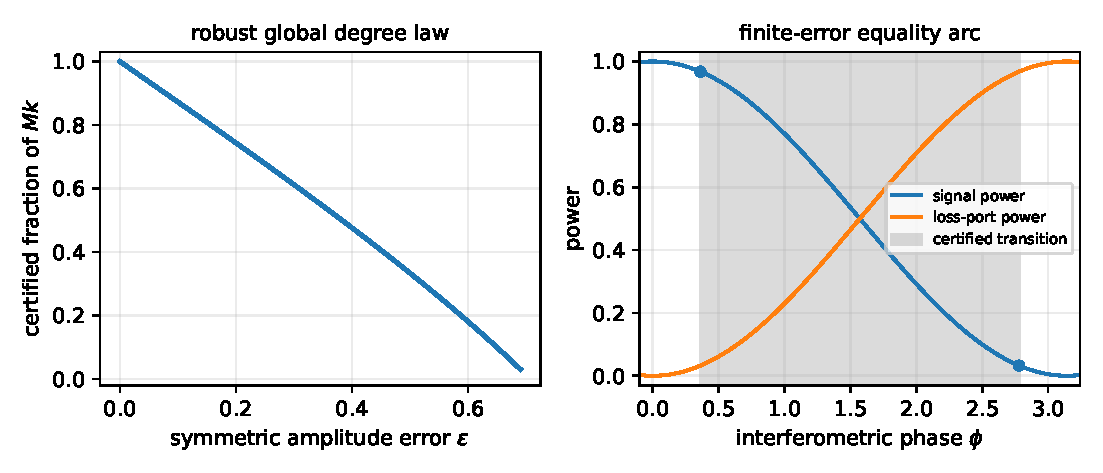
\includegraphics[width=\linewidth]{figures/routing_law.pdf}
 \caption{Left: certified fraction of the exact degree law for symmetric
 amplitude error.  Right: an equality arc of the interferometric family;
 both delay integrals equal their geometric lower bounds on the shaded
 interval.}
 \label{fig:routing}
\end{figure}

\section{From scattering data to a certificate}

The theorem can be evaluated from boundary-frequency measurements.  It does
not require pole fitting, analytic continuation or knowledge of an internal
realization.

Suppose only the signal-sector block
$G(\theta)=R_AS(\theta)J$ is measured and the full passive model admits a
unitary completion.  Let $\widehat G$ satisfy an operator-norm error bound
\begin{equation}\label{eq:measurementerror}
 \onorm{(\widehat G(\theta)-G(\theta))V}\leq\eta_\theta.
\end{equation}
At a nominal pass point define
$g_p=\sigma_{\min}(\widehat G(p)V)$, and at a nominal stop point define
$g_s=\onorm{\widehat G(s)V}$.  Weyl's singular-value perturbation bound and
unitarity give certified actual leakages
\begin{equation}\label{eq:inflatederrors}
 \varepsilon_p^{\mathrm{cert}}
 =\sqrt{1-\min\{1,[g_p-\eta_p]_+\}^2},
 \qquad
 \varepsilon_s^{\mathrm{cert}}
 =\min\{1,g_s+\eta_s\}.
\end{equation}
Indeed $C^*C=I-G^*G$ on the selected inputs.  Substituting the inflated
errors into \eqref{eq:alpha} produces a rigorous lower bound.  The
certificate remains useful whenever
\[
 \arcsin\varepsilon_p^{\mathrm{cert}}
 +\arcsin\varepsilon_s^{\mathrm{cert}}<\frac{\pi}{2}.
\]

For each adjacent transition the measured angular separation $\Delta$ then
adds the peak-delay certificate \eqref{eq:localpeak}.  Thus separation is
not needed to infer a global degree cost, but it decides how concentrated
the unavoidable memory must be.  This cleanly separates two experimental
questions:
\[
 \text{how many switches?}\ \longrightarrow\ \text{total degree},
 \qquad
 \text{how narrow are they?}\ \longrightarrow\ \text{peak delay}.
\]

\section{Implication for passive quantum reservoirs}

In a linear passive quantum network, $S$ routes bosonic input fields among
output ports while preserving canonical commutation relations
\cite{GoughJames2009,GoughZhang2015}.  Choose $R_A$ as the sector coupled to
the observed system and $R_B$ as an auxiliary or loss sector.  A rank-$k$
bath subspace routed to $A$ at one frequency and to $B$ at another changes
which environmental directions reach the system.

For a bath spectral matrix $J_B(\omega)$ with
$j_-I\preceq J_B\preceq j_+I$, the weak-coupling contribution through the
signal block is
\begin{equation}\label{eq:kossakowski}
 \Gamma_G(\omega)=G(\omega)J_B(\omega)G(\omega)^*.
\end{equation}
At a pass point with amplitude leakage $\varepsilon_p$, every selected unit
input has signal norm at least $\sqrt{1-\varepsilon_p^2}$; at a stop point
it has signal norm at most $\varepsilon_s$.  Hence the filtered rate scale
changes from at least $j_-(1-\varepsilon_p^2)$ to at most
$j_+\varepsilon_s^2$ along the selected directions.  Repeating this switch
$M$ times forces the memory and delay costs above.  The rate statement uses
the standard weak-coupling interface \cite{Davies1974}; the scattering
theorem itself is independent of a Markov approximation.

This gives a precise operational reading: moving a quantum noise subspace
back and forth across a spectral system--environment boundary cannot be done
by a memoryless passive box.  The word ``memory'' refers to internal dynamical
degree and Wigner--Smith dwell time, not directly to thermodynamic work or
Landauer energy.  That distinction follows the resource-boundary outlook of
\cite{ErikssonCut2026} without importing its broader conjectures into the
present theorem.

\section{Reproducible adversarial audit}

The proof is analytic.  Numerical experiments are designed to attack its
interfaces, not to establish it.  The public artifact contains a generator,
a frozen JSON ledger and an independent verifier.

\begin{table}[t]
\centering
\caption{Certificate layers.  Ratios must not exceed one.}
\label{tab:audit}
\begin{tabular}{@{}lrrl@{}}
\toprule
Audit & trials/cases & worst ratio & result\\
\midrule
finite-error equality arcs & 15 & $1.000000$ & equality\\
exact cyclic families & 4 & $1.000000$ & equality\\
positive block, trace norm & 2048 & $0.845291$ & pass\\
positive block, operator norm & 2048 & $0.971240$ & pass\\
random Potapov paths & 512 & $0.999817$ & pass\\
\bottomrule
\end{tabular}
\end{table}

The finite-error suite uses $k\in\{1,2,4\}$, orders
$M\in\{3,5,7\}$ and asymmetric as well as symmetric errors.  It checks the
endpoint overlap, principal angle, arc width and both integrated delays
against exact closed forms.  The cyclic suite checks degree and total action
at orders up to seven and rank four.

The positive-block test draws 2,048 dense complex positive matrices of sizes
three through twelve and random projections of every admissible type.  It
separately attacks
\[
 \frac{2\|(I-P)QP\|_1}{\tr Q}\leq1,
 \qquad
 \frac{2\|(I-P)QP\|_{\mathrm{op}}}{\lambda_{\max}(Q)}\leq1.
\]
The path test draws 512 matrix inner products with up to twelve independent
rank-one Blaschke--Potapov factors, random subspaces of ranks one through
three and independent frequency arcs.  It compares the endpoint
trace-angular Grassmann distance with half the adaptively integrated
Wigner--Smith trace.  The most adversarial draw reaches $0.999817$ of the
bound without crossing it.

The complete replay is:
\begin{center}
\url{https://github.com/lluiseriksson/finite-sample-spectral-certificates/tree/research/robust-spectral-routing}
\end{center}
and the principal commands are
\begin{verbatim}
python research/routing_speed_limit_certificate.py
python verification/verify_routing_speed_limit.py
python verification/run_routing_speed_limit_release_checks.py
\end{verbatim}

\section{Relation to existing bounds and priority boundary}

Every ingredient used in the proof has a classical life.  Wigner and Smith
introduced phase and lifetime delay \cite{Wigner1955,Smith1960}; modern
multiport formulations connect the matrix to field-energy overlaps and
frequency sensitivity \cite{PatelMichielssen2021}.  Canonical angles and
unitarily invariant Grassmann metrics are established matrix geometry
\cite{QiuZhangLi2005,EdelmanAriasSmith1998}.  McMillan degree and rational
inner factorization are standard realization theory
\cite{McMillan1952,Potapov1955}.  Geometric quantum speed limits provide a
useful temporal analogy \cite{AnandanAharonov1990}.

Several nearby theories answer different questions.  Bode--Fano bounds
integrate logarithmic mismatch against load-dependent pole data and their
multiport extensions address broadband matching
\cite{Fano1950,Chen1989}.  Boundary and tangential interpolation prescribe
complex values or angular derivatives and study solvability or minimal
degree \cite{BallKang1990,BallBolotnikov2017,Bolotnikov2016}.  Quantum filter
functions quantify noise transfer for specified control protocols
\cite{CerfontaineEtAl2021}.  None of these results, in the sources audited
here, states the displayed leakage-only chain
\[
 \begin{aligned}
 &\text{approximate routing between orthogonal output sectors}\\
 &\quad\Longrightarrow\text{Grassmann motion}
 \Longrightarrow\text{positive Wigner--Smith action}\\
 &\quad\Longrightarrow\text{McMillan degree},
 \end{aligned}
\]
with the sharp constants of \cref{thm:local,cor:degree}.  This is the
specific novelty claim.  We do not claim new Grassmann geometry, a new
Wigner--Smith definition, a replacement for Bode--Fano theory or a complete
solution of robust rational interpolation.

The sequence of preceding papers had progressively narrower comparison
loopholes.  Noncommuting filters supplied an irreducible construction
\cite{ErikssonMIMO2026}; passive reservoir filtering converted its amplitude
gap into a decoherence-rate gap and exposed a delay price
\cite{ErikssonReservoir2026}; the exact calibration-memory law replaced a
restricted comparator by a universal rational-inner degree bound
\cite{ErikssonMemory2026}.  The present paper removes the exact-calibration
requirement for ordered pass/stop data and extends the action statement
beyond rational networks.

\section{Scope, failure modes and open problems}

\begin{limitation}[Positive Wigner--Smith class]
Arbitrary unitary scattering matrices can have signed proper delays.  The
sharp factor two and the degree identity apply to the positive class,
including causal rational inner matrices in the disk convention used here.
For signed paths the absolute-action variant after \cref{cor:degree} is the
valid statement.
\end{limitation}

\begin{limitation}[Fixed input subspace]
The same rank-$k$ input subspace is tracked along each certified arc.  If the
input directions are allowed to change adversarially from sample to sample,
the network need not move a common subspace.  A useful extension would add a
measured correspondence or transport cost between changing input frames.
\end{limitation}

\begin{limitation}[Complementary sectors]
The clean angle formula uses $R_A+R_B=I$.  Additional unmonitored outputs can
be included in either sector.  If they are left outside both, their leakage
must be measured and included in a three-sector angle bound.
\end{limitation}

\begin{limitation}[Degree is not hardware energy]
McMillan degree, trace delay and proper delay quantify dynamical memory.
They do not by themselves determine fabrication volume, temperature,
initialization cost or dissipated work.  Such conversions require a physical
realization model.
\end{limitation}

The most promising extensions are a measure-valued version for singular
inner factors, routing among more than two sectors through a target-subspace
graph, and statistical confidence regions for experimentally reconstructed
operator norms.  A second direction is synthesis: characterize all rational
inner matrices attaining the local equalities.  The proof shows they must
simultaneously saturate the Grassmann geodesic and both positive-block
inequalities, strongly constraining their Wigner--Smith generator.

\section{Conclusion}

Approximate spectral routing has a compulsory memory cost.  Each transition
of a rank-$k$ input subspace between complementary output sectors covers a
robust canonical angle
\[
 \alpha=\left[\frac\pi2-\arcsin\varepsilon_p
                         -\arcsin\varepsilon_s\right]_+,
\]
and positive Wigner--Smith dynamics must spend at least $2k\alpha$ of trace
action and $2\alpha$ of largest-eigenvalue action on that arc.  Disjoint
transitions add.  Rational inner networks have only $2\pi n$ total trace
action, so $M$ alternating pass/stop pairs force
\[
 n\geq\frac{2Mk}{\pi}\alpha.
\]
The zero-error law $n\geq Mk$ and both local finite-error delay laws are
sharp in every rank.  The certificate needs only leakage, ordering and
frequency separation measured on the physical boundary.  It therefore
closes the gap between exact topological calibration counts and finite-error
laboratory data while preserving an architecture-independent conclusion.

\bibliographystyle{unsrt}
\bibliography{references}

\end{document}
